
%%%%%%%%%%%%%%%%%%%%%%% file typeinst.tex %%%%%%%%%%%%%%%%%%%%%%%%%
%
% This is the LaTeX source for the instructions to authors using
% the LaTeX document class 'llncs.cls' for contributions to
% the Lecture Notes in Computer Sciences series.
% http://www.springer.com/lncs       Springer Heidelberg 2006/05/04
%
% It may be used as a template for your own input - copy it
% to a new file with a new name and use it as the basis
% for your article.
%
% NB: the document class 'llncs' has its own and detailed documentation, see
% ftp://ftp.springer.de/data/pubftp/pub/tex/latex/llncs/latex2e/llncsdoc.pdf
%
%%%%%%%%%%%%%%%%%%%%%%%%%%%%%%%%%%%%%%%%%%%%%%%%%%%%%%%%%%%%%%%%%%%


\documentclass[runningheads,a4paper]{llncs}

\usepackage{amssymb}
\setcounter{tocdepth}{3}
\usepackage{graphicx}
\usepackage[utf8]{inputenc}

\usepackage{url}
\urldef{\mailsa}\path|{rodrigo.g.branco,dmbpaiva,istela}@gmail.com|    
\newcommand{\keywords}[1]{\par\addvspace\baselineskip
\noindent\keywordname\enspace\ignorespaces#1}

\usepackage{epstopdf}

\begin{document}

\mainmatter  % start of an individual contribution

% first the title is needed
\title{AccTrace: Acessibilidade nas fases de Engenharia de Requisitos, Projeto e Codificação de Software}

% a short form should be given in case it is too long for the running head

%VERIFICAR
\titlerunning{AccTrace}

% the name(s) of the author(s) follow(s) next
%
% NB: Chinese authors should write their first names(s) in front of
% their surnames. This ensures that the names appear correctly in
% the running heads and the author index.
%
\author{Rodrigo Gonçalves de Branco%
%\thanks{Please note that the LNCS Editorial assumes that all authors have used
%the western naming convention, with given names preceding surnames. This determines
%the structure of the names in the running heads and the author index.}%
\and Débora Maria Barroso Paiva \and Maria Istela Cagnin}

%VERIFICAR
\authorrunning{AccTrace}
% (feature abused for this document to repeat the title also on left hand pages)

% the affiliations are given next; don't give your e-mail address
% unless you accept that it will be published
\institute{Faculdade de Computação - FACOM\\
Universidade Federal de Mato Grosso do Sul - UFMS\\
Cidade Universitária, Campo Grande - MS, Brasil\\
\mailsa\\
\url{http://facom.ufms.br/}}

%
% NB: a more complex sample for affiliations and the mapping to the
% corresponding authors can be found in the file "llncs.dem"
% (search for the string "\mainmatter" where a contribution starts).
% "llncs.dem" accompanies the document class "llncs.cls".
%

\toctitle{Lecture Notes in Computer Science}
\tocauthor{Authors' Instructions}
\maketitle


\begin{abstract}
The abstract should summarize the contents of the paper and should
contain at least 70 and at most 150 words. It should be written using the
\emph{abstract} environment.
\keywords{Accessibility, Requirement Traceability, Software Development
Process, CASE Tool}
%\keywords{We would like to encourage you to list your keywords within
%the abstract section}
\end{abstract}


\section{Introdução}

A Internet se consolidou como um dos principais meios de comunicação, disseminação da informação e fornecimento de serviços nos dias atuais, sendo que determinados tipos de informações são disponibilizados apenas através deste meio. Fornecer o acesso a estas informações para uma imensa variedade de dispositivos, com tecnologias e especificações diferentes, se tornou um desafio. E, principalmente, pessoas com necessidades especiais, devido a suas características inerentes, necessitam de produtos especialmente desenvolvidos para este fim.

Construir produtos acessíveis não é uma tarefa fácil e este assunto é alvo de muitas pesquisas \cite{lazar:04,brajnik:06,zeng:05}, existindo propostas específicas para integrar usabilidade e acessibilidade aos processos de Engenharia de Software \cite{springerlink:10.1007/978-3-642-02713-0,maia:10}. Contudo, devido a fatores como a recente exposição do tema nos meios de comunicação e a deficiência no treinamento e formação  dos desenvolvedores, muitos deles sequer sabem como codificar para tornar seus produtos acessíveis \cite{1630123,alves:11}.

A utilização de ferramentas que apóiam os profissionais na construção de boas soluções acessíveis é muito comum, pois estas aumentam a produtividade e diminuem o esforço necessário. Estas ferramentas podem variar entre ferramentas CASE, IDEs, frameworks, simuladores, validadores, avaliadores e até mesmo uma mistura destas citadas. Contudo, pesquisas mostram que as ferramentas disponíveis deixam a desejar no quesito de apoio à acessibilidade \cite{Trewin:2010:ACT:1805986.1806029}.

A situação é agravada pela constatação de que, apesar de existirem vários estudos sobre rastreabilidade de requisitos genéricos \cite{5970169,292398,5485417,6405269}, poucos estudos têm indicado como ocorre a evolução dos requisitos de acessibilidade durante o processo de desenvolvimento das aplicações web \cite{analuizadias:2010}, e como os desenvolvedores utilizarão essa informação para construir o produto.

Este artigo apresenta o AccTrace, uma ferramenta CASE desenvolvida como um
plugin do Eclipse para, através da rastreabilidade dos requisitos de
acessibilidade, entregar ao desenvolvedor informações relevantes para a
construção de um produto acessível. O AccTrace foi baseado em um processo de
desenvolvimento de softwares que incluía tarefas de acessibilidades baseado na
ISO 12207, chamado MTA \cite{maia:10}. Durante o processo de desenvolvimento do
software, as referências entre requisitos e modelos UML, juntamente com a nova
abordagem de especificar quais serão as técnicas de implementação de
acessibilidade para estes relacionamentos, resultam em um comentário
personalizado no código fonte, que é recuperado em tempo real detalhando as
informações descritas anteriormente.

\subsection{Exemplo Motivacional}

A rastreabilidade dos requisitos geralmente é feita utilizando matrizes de
rastreabilidade \cite{guo:2009:OBI:1681515.1682933}. Contudo, nas abordagens tradicionais, os
requisitos de acessibilidade não são diferenciados dos outros requisitos. Desta
forma, a implementação de tais requisitos não se torna explícita.
Desenvolvedores experientes podem não encontrar problemas na implementação, mas
desenvolvedores iniciantes podem não ter o mesmo sucesso.

É certo que o documento WCAG 2.0 pode e deve ser usado como documento de
referência, pois ele contém critérios de sucesso, técnicas para implementação,
etc. Contudo, este documento não é de fácil leitura para iniciantes,
principalmente no que tange encontrar a informação necessária. Por este motivo,
inclusive, que normalmente o documento é usado para avaliar e validar produtos
prontos.

O desenvolvedor seria beneficiado caso a informação de o que deve ser feito, no
que tange acessibilidade, estivesse disponível. Isto é exatamente o que nossa
abordagem tenta resolver.

\section{Trabalhos Relacionados}

Os trabalhos anteriores relacionados a este podem ser divididos em três grupos:
Acessibilidade no Processo de Desenvolvimento de Software, Rastreabilidade de
Requisitos e Ontologias para o Mapeamento do Domínio.

\subsection{Acessibilidade no Processo de Desenvolvimento de Software}

O tema Acessibilidade no Processo de desenvolvimento de software ainda
é pouco explorado. Maia \cite{maia:10} propôs  integrar usabilidade e
acessibilidade aos processos de Engenharia de Software criando o MTA (Modelo de
Tarefas de Acessibilidade), um modelo de desenvolvimento, baseado na norma ISO/IEC 12207, aplicável
ao WCAG, que permite o apoio ferramental ao modelo.

\subsection{Rastreabilidade de Requisitos}

Diversos estudos que dizem respeito ao rastreamento de requisitos podem ser
encontrados na literatura.

 Em contrapartida, podem ser encontrados diversos
estudos que dizem respeito ao rastreamento de requisitos
\cite{5970169,292398,5485417,6405269}, 

\subsection{Ontologias para o Mapeamento do Domínio}

bem como encontrar estudos que utilizam
ontologias para o mapeamento do domínio no processo de desenvolvimento ou na
rastreabilidade dos requisitos \cite{5223183,6511842,4148940,5362244}. Contudo,
não foi encontrado na literatura estudos específicos sobre a rastreabilidade de
requisitos de acessibilidade durante o processo de desenvolvimento de software.

\section{Abordagem}

O AccTrace utiliza como escopo o Processo de Desenvolvimento de Software do MTA
\cite{maia:10}, e os subprocessos 4 (Análise de Requisitos do Software), 5
(Projeto de Software) e 6 (Construção do software). Como o escopo deste trabalho
diz respeito a rastreabilidade dos requisitos de acessibilidade e suas técnicas
de implementaçÕ, as tarefas de testes, presentes no Subprocesso 6, não serão
levadas em consideração. 

Neste trabalho, propõe-se que os artefatos gerados pelo MTA aqui utilizados e os
artefatos novos introduzidos estejam em um formato legível por máquina, para
persistência de tais informações no modelo de dados da ferramenta.

A Figura \ref{fig:figmagica} apresenta a abordagem escolhida e mostra como,
partindo da Engenharia de Requisitos e chegando na construção do software,
a rastreabilidade dos requisitos e das técnicas de implementação de
acessibilidade é alcançada.

\begin{figure}[h!]
\centering
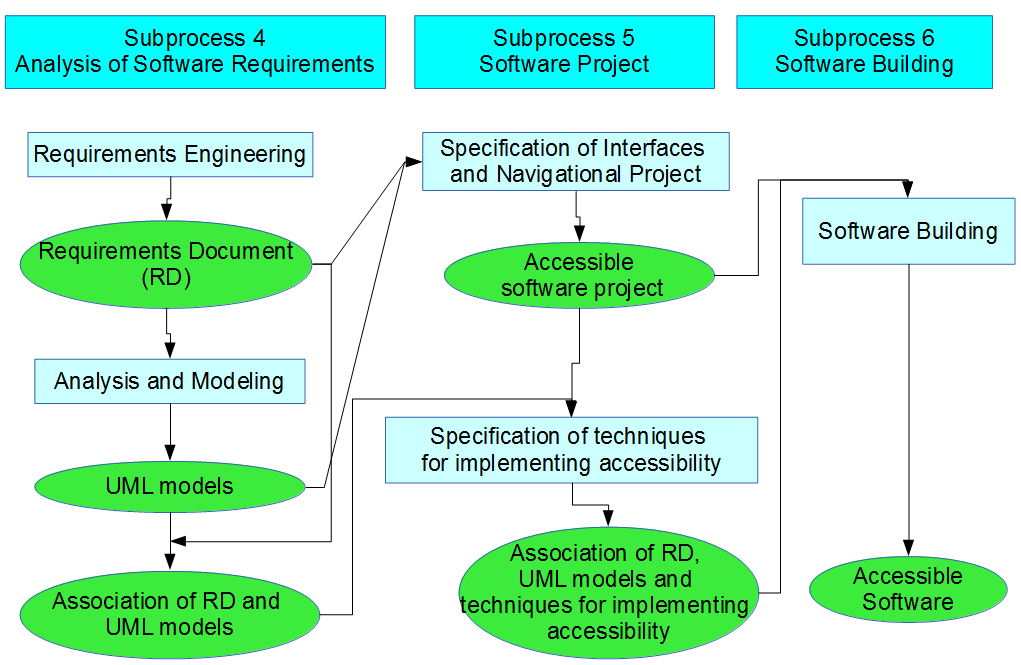
\includegraphics[scale=0.25]{img/figuramagica.png}
\caption{Detalhamento dos Subprocessos do MTA para prover a rastreabilidade dos
requisitos de acessibilidade de acordo com a abordagem adotada neste trabalho}
\label{fig:figmagica}
\end{figure}

\subsection{Especialista em Acessibilidade}

O MTA apresenta o papel de Especialista em Acessibilidade, fundamental em todas
as etapas das tarefas de acessibilidade. Assim como o MTA, o AccTrace supõe que
a equipe de desenvolvimento possui tal persona, cujo papel é identificar os
requisitos de acessibilidade, bem como apresentar a associação dos requisitos,
modelos UML e técnicas de implementação de acessibilidade, que serão explicadas
adiante.

\subsection{Subprocesso 4 - Análise de Requisitos de Software}

O Subprocesso 4 traz duas tarefas de acessibilidade (\textbf{Estabelecer e
Documentar os Requisitos de Acessibilidade do Software} e \textbf{Avaliar os
Requisitos de Acessibilidade do Software}). A saída da tarefa {Avaliar os
Requisitos de Acessibilidade do Software} gera o artefato \textbf{Documento de
requisitos de acessibilidade do software avaliados e aprovados}.

A construção dos modelos UML na etapa Análise e Modelagem, conforme apresentado
na Figura \ref{fig:figmagica}, recebe como entrada o artefato \textbf{Documento
de Requisitos do software avaliado e aprovado}, para que a associação dos
requisitos e modelos seja efetuada.

\subsection{Subprocesso 5 - Projeto de Software}

O Subprocesso 5 introduz três tarefas de acessibilidade (\textbf{Projetar
Interfaces Externas Acessíveis}, \textbf{Realizar Projeto Navigacional
Acessível} e \textbf{Avaliar a Acessibilidade do Projeto de Software}). O
Documento de Requisitos e os Modelos UML são utilizados para realizar a
especificação de Interfaces e do Projeto Navegacional, gerando o artefato
\textbf{Projeto de Software Acessível}. Neste momento, é possível especificar
quais serão as técnicas de implementação de acessibilidade e associá-las aos
requisitos e modelos UML.

\subsection{Subprocesso 6 - Construção do Software}

O Subprocesso 6 possui duas tarefas importantes para o escopo deste trabalho
(\textbf{Especificar Técnicas para Implementação da Acessibilidade da
Interface e do Código} e \textbf{Codificar e documentar cada unidade de software
de acordo com as técnicas de acessibilidade}). Para a rastreabilidade, a
especificação das técnicas de implementação de acessibilidade já foram feitas no
Subprocesso 5, faltando aqui efetuar a documentação para as mesmas. A etapa
\textbf{Construção do Software} (Figura \ref{fig:figmagica}) utilizará os
artefatos \textbf{Projeto de Software Acessível} e as especificações de técnicas
de implementação de acessibilidade para finalmente permitir a construção do
Software acessível.

\section{Detalhes de Implementação}

O AccTrace foi desenvolvido utilizando as seguintes tecnologias:

\begin{itemize}
  \item MTA;
  \item Eclipse Juno - IDE;
  \item Requirement Designer v0.8.0 - Gerenciamento de Requisitos;
  \item UML Designer v2.1.0 - Modelagem UML;
  \item UML to Java Generator v1.0.2 - Geração de código;
  \item Java JRE e JDK 1.7 - Desenvolvimento da ferramenta;
  \item Projeto Aegis - ontologia de mapeamento do domínio de acessibilidade (usando o WCAG 2.0).
\end{itemize}

O Eclipse é uma plataforma madura e foi escolhido como IDE por vários motivos. Ele
serve como base para diversos produtos e tecnologias baseadas em uma IDE, provendo
uma API para facilitar a integração. O desenvolvimento de plugins para o Eclipse é feito diretamente na IDE,
de forma prática e transparente, tendo ampla documentação a respeito. A linguagem
utilizada para o desenvolvimento do plugin é a linguagem Java, assim como o código
gerado pelo plugin de exportação.

Os plugins de gerenciamento de requisitos (Requirement Designer) e modelagem (UML Designer) são desenvolvidos pela Obeo e são interoperáveis, portanto, para permitir uma integração suave entre as ferramentas, o plugin escolhido para geração de código foi o UML to Java Generator, desenvolvido pela
mesma empresa. Todos estes plugins, assim como o AccTrace, persistem seus dados como arquivos RDF modelados com o formato EMF. Os plugins são disponibilizados sob a licença Eclipse Public License v1.0, assim como a própria IDE. Dessa forma, é possível estudar, alterar e customizar seus componentes para atingir os objetivos do trabalho.

O Projeto Aegis \cite{aegis:13} define uma ontologia de acessibilidade, descrita no padrão OWL 1.0, e vai além de realizar o mapeamento dos conceitos de acessibilidade e cenários. Os arquivos disponibilizados mapeiam o modelo WCAG 2.0 (incluindo técnicas de implementação, critérios de sucesso e falha, etc), leitores de tela, navegadores textuais, lentes de aumento, WAI/ARIA, entre outros.

A Figura \ref{fig:association} mostra o comportamento e relacionamento das ferramentas, tecnologias
e atores envolvidos no desenvolvimento do produto.

\begin{figure}[h!]
\centering
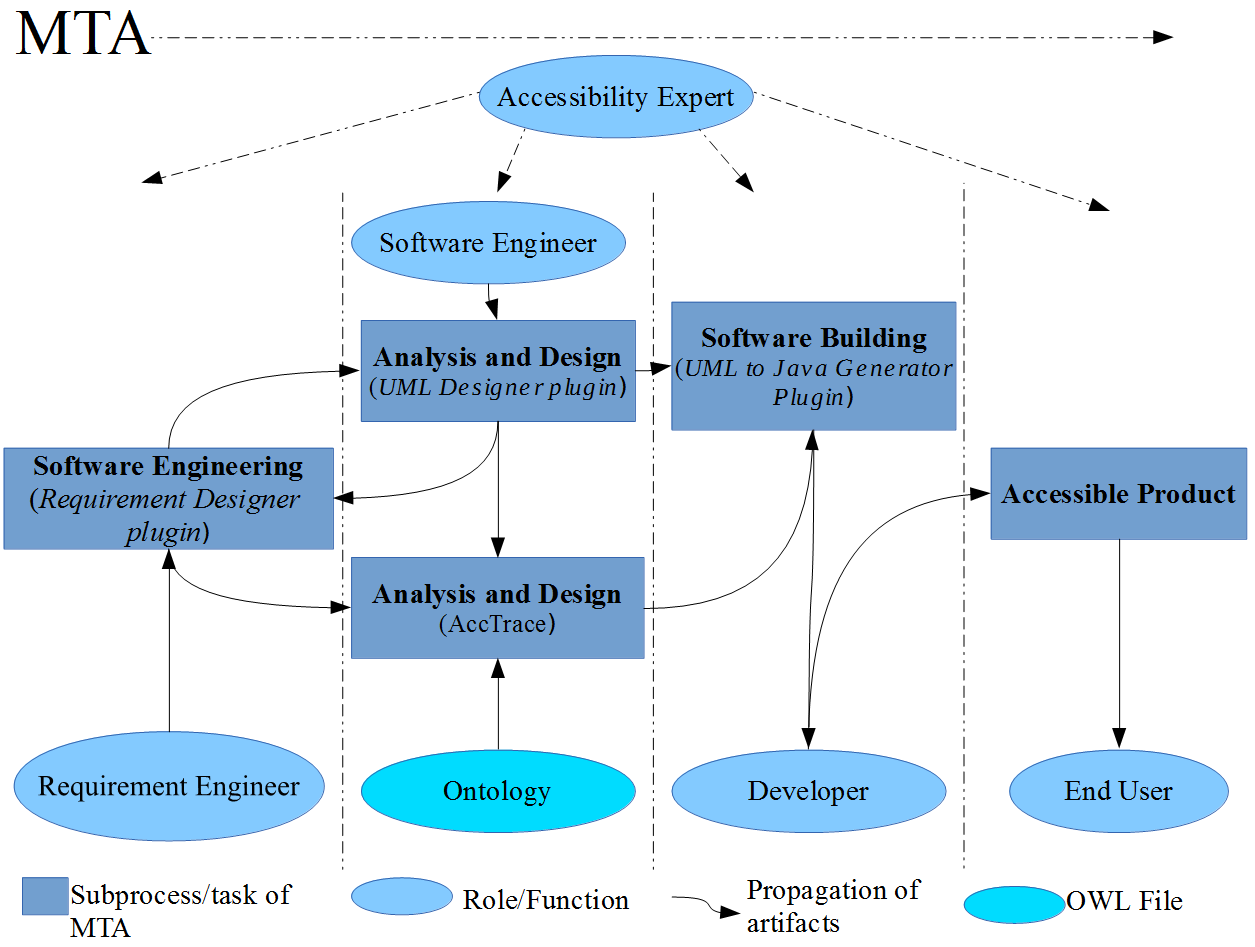
\includegraphics[scale=0.25]{./img/developmentNew2.png}
\caption{Associação das ferramentas e atores no contexto do trabalho}
\label{fig:association}
\end{figure}

Podemos interpretar a Figura \ref{fig:association} da seguinte forma:

\begin{itemize}
  \item O MTA é o processo de desenvolvimento e deve permear todas as fases do processo;
  \item O especialista em acessibilidade (Accessibility Expert) deve participar das fases de
desenvolvimento especificadas no MTA;
  \item Os requisitos devem ser coletados e informados na fase de engenharia de requisitos
(utilizando a ferramenta Requirement Designer) e os modelos e artefatos UML
devem ser gerados (utilizando a ferramenta UML Designer). O especialista em
acessibilidade deve auxiliar a alimentação destes dados, filltrando os requisitos de
acessibilidade para que eles sejam associados aos modelos UML (utilizando a ferramenta
Requirement Designer);
  \item O AccTrace recupera as associações dos requisitos e modelos UML, permitindo que o especialista especifique as técnicas de implementaçãoo de acessibilidade para cada uma das associações. As técnicas, diretrizes, abordagens, dentre outros estão armazenadas em arquivos OWL embutidos na ferramenta;
  \item A ferramenta de geração de código produzirá o código stub a partir dos modelos
UML, adicionando as referências às associações de acessibilidade quando necessário;
  \item Os desenvolvedores refinam o cóodigo até que o mesmo esteja apto a se tornar o
produto acessível que será entregue.
\end{itemize}

A ferramenta possui três visões principais, de acordo com a Figura \ref{fig:acctrace}. 

\begin{figure}[h!]
\centering
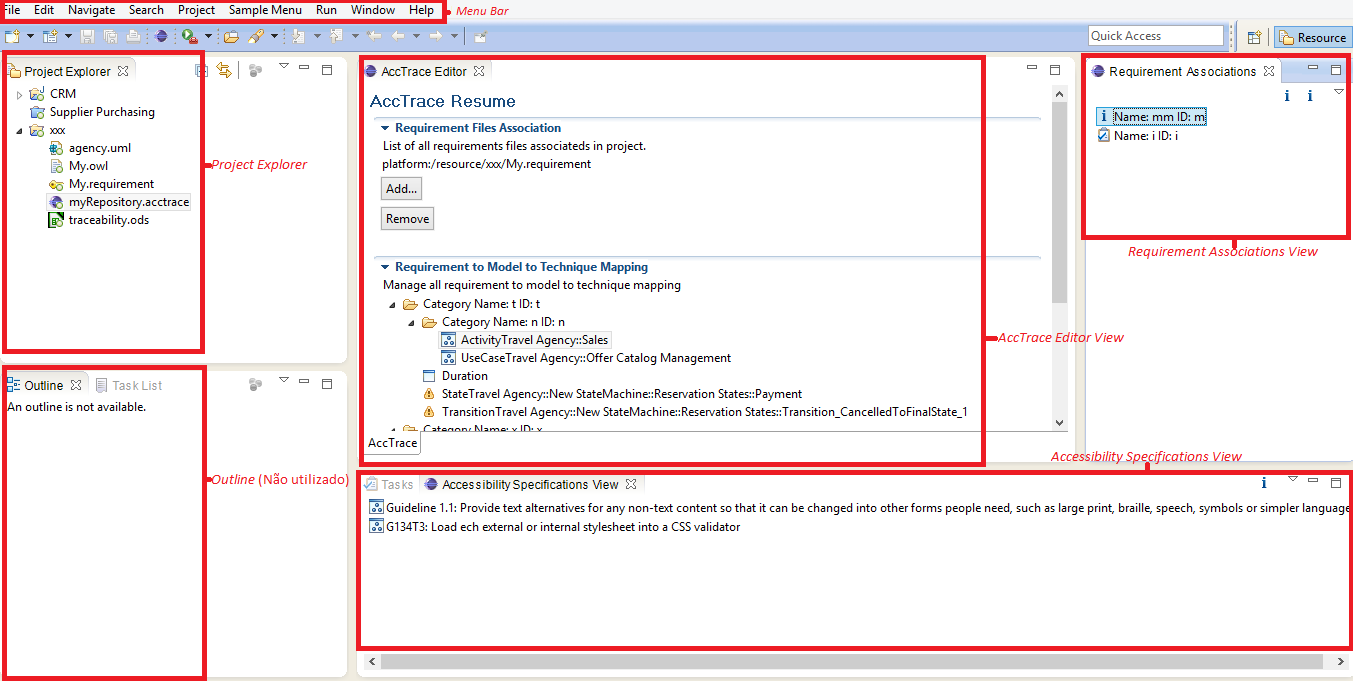
\includegraphics[scale=0.26]{./img/acctrace.png}
\caption{Visualização da ferramenta AccTrace na tela principal do
Eclipse}
\label{fig:acctrace}
\end{figure}

No editor (AccTrace Editor) é possível alterar os repositórios dos requisitos e gerar as associações entre os modelos UML, requisitos e técnicas de implementação. Na visão
dos requisitos (Requirement Associations) é possível visualizar quais requisitos associados
ao modelo UML foram selecionados no editor. Na visão das técnicas já vinculadas
(Accessibility Specifications View) é possível visualizar as técnicas de implementação já
associadas, de acordo com o modelo UML selecionado no editor e o requisito de acessibilidade
selecionado na visão dos requisitos. Além disso, é possível remover as técnicas de
implementação associadas. As três visões são importantes para o correto funcionamento
da ferramenta.

Uma vez selecionado o modelo UML e o requisito, é possível efetuar a associação da
técnica de implementação de acessibilidade, clicando com o botãoo direito do mouse em
cima do modelo UML, conforme demonstrado na Figura \ref{fig:rightclick}.

\begin{figure}[h!]
\centering
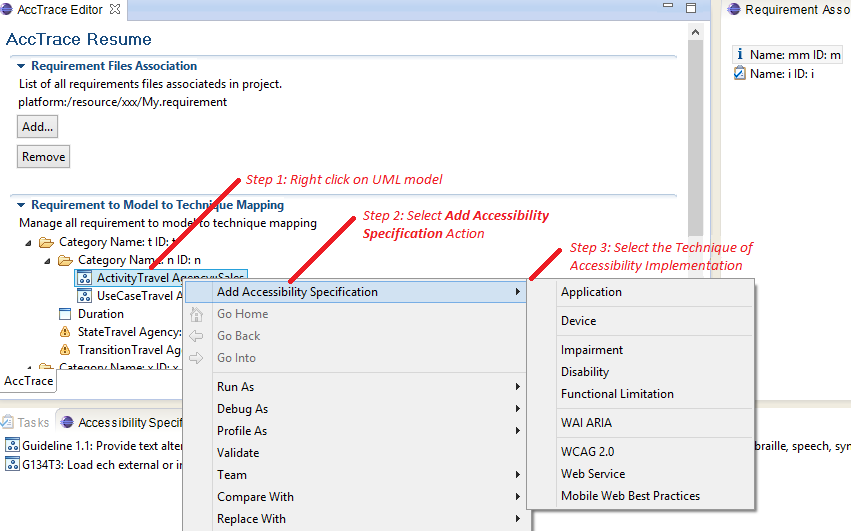
\includegraphics[scale=0.25]{./img/rightclick.png}
\caption{Procedimento para efetuar a associação da técnica de implementação de
acessibilidade}
\label{fig:rightclick}
\end{figure}

A hieraquia dos elementos da ontologia, presentes nos arquivos OWL, são apresentados em alto nível na Figura \ref{fig:ontologyrelationship}.

\begin{figure}[h!]
\centering
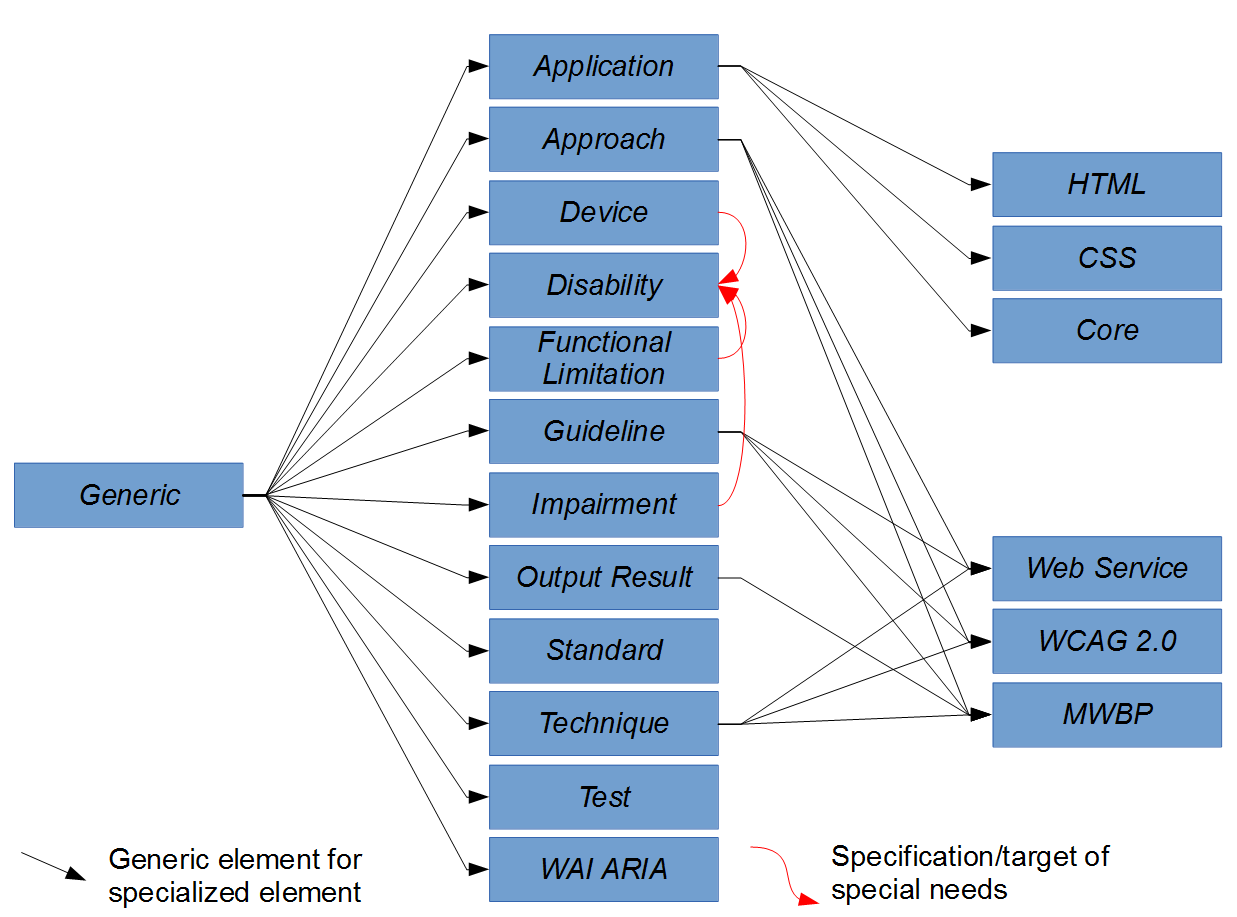
\includegraphics[scale=0.18]{./img/ontologyrelationship.png}
\caption{Relacionamento entre os elementos da ontologia (Elementos retirados
da ontologia)}
\label{fig:ontologyrelationship}
\end{figure}

Após os requisitos, modelos UML e as técnicas de implementação serem associadas, é possível gerar a matriz de rastreabilidade.
Neste trabalho foi utilizado o Apache ODF Toolkit para geração do documento de rastreamento com formato Open-Document Spreadsheet file format (ODS), através da API de alto nível Simple. No documento, são geradas três planilhas: Requisitos \textit{versus} Modelos, Requisitos \textit{versus} Técnicas e Modelos \textit{versus} Técnicas. A planilha Requisitos \textit{versus} Modelos lista uma matriz de todos os Requisitos associados aos respectivos modelos. Requisitos que não estão associados a um modelo também são listados. Essa situação está prevista
justamente para identificar problemas na associação que devam ser corrigidos. Para as
planilhas Requisitos \textit{versus} Técnicas e Modelos \textit{versus} Técnicas, apenas os objetos que
estão efetivamente referenciados na ferramenta são listados.

Por fim, é possível efetuar a geração de código utilizando o plugin UML to Java Generator, que por sua vez utiliza o ponto de extensão do plugin Acceleo.
O plugin UML to Java Generator foi especialmente modificado para que reconhecesse as associações entre Requisitos, Modelos UML e técnicas de implementação de acessibilidade, gerando comentários personalizados nos escopos corretos das classes de acordo com a expressão regular Java demonstrada a seguir:

\medskip

\noindent
\begin{verbatim}
String regex = "//!ACCTRACE!(/)?([^/\\\\0#]+(/)?)+#([^\\*\\*/])+";
\end{verbatim}
%
\noindent

A expressão regular foi construída de modo a permitir, através de uma string pré-definida, a recuperação do arquivo Acctrace,
bem como do elemento de associação referenciado. O comentário personalizado foi projetado de forma a não interfirir em outros
comentários da linguagem. Iniciando pelas barras duplas (//), foi definido um
identificador que tem a intenção de ser único (!ACCTRACE!), e o próprio ID do recurso RDF possui o caracter ``\#'', que é usado para separador entre
o recurso (arquivo a ser aberto) e o elemento a ser resgatado (no caso, a
associação criada entre o requisito e o modelo UML). A opção de se
utilizar um comentário de linha (ao invés de comentários de bloco, usados por exemplo pela documentação JavaDoc) decorreu do fato
do comentário descrito ser incluído dentro do corpo da classe e métodos, e caso
o programador decida comentar o trecho de código inteiro, esse comentário não
atrapalharia essa operação.

A Figura \ref{fig:commentrecovery} mostra os passos necessários para recuração das informações de um comentário AccTrace, e a Figura \ref{fig:commentview}
mostra a visão das informações recuperadas na visão específica para este fim no Eclipse.

\begin{figure}[h!]
\centering
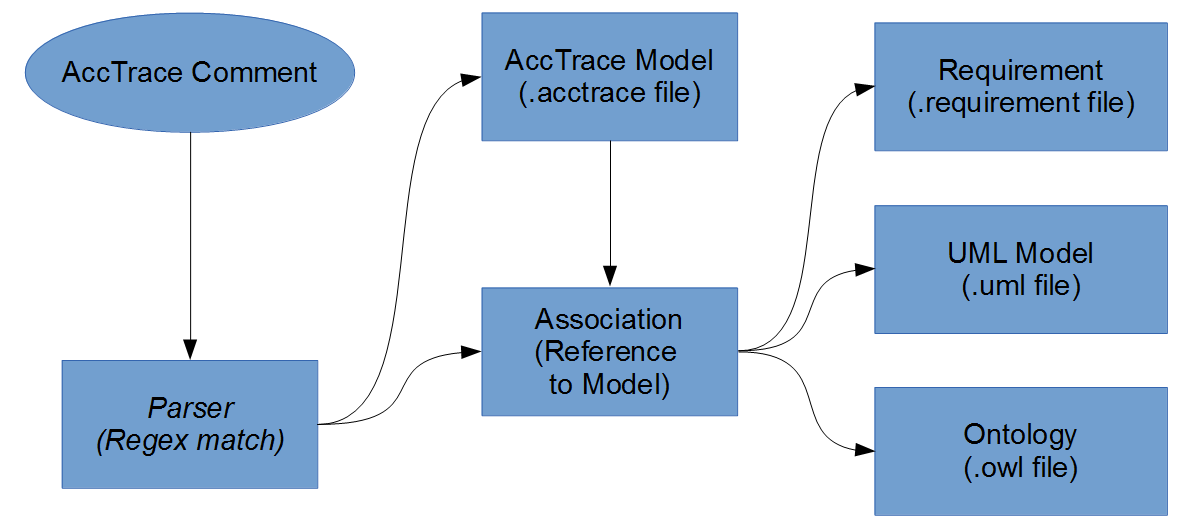
\includegraphics[scale=0.17]{./img/commentrecovery.png}
\caption{Passos para recuperação das informações relevantes através de um
comentário padrão AccTrace}
\label{fig:commentrecovery}
\end{figure} 

\begin{figure}[h!]
\centering
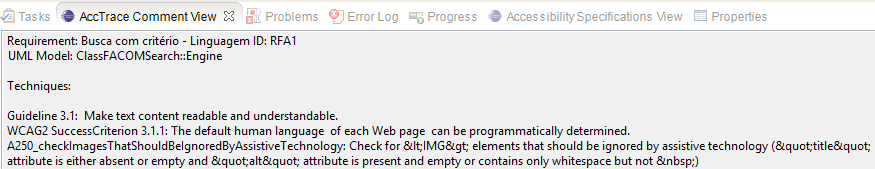
\includegraphics[scale=0.45]{./img/commentview.png}
\caption{Explicitação do comentário selecionado}
\label{fig:commentview}
\end{figure}

\section{Avaliação - Prova de Conceito}

Para validar a efetividade da abordagem proposta, foi criado um projeto simples como prova de conceito, utilizando o MTA, o AccTrace e os outros recursos relacionados neste trabalho. O objetivo desta prova de conceito foi verificar se o AccTrace:

\begin{itemize}
  \item Permite a verificação da relação entre os requisitos e casos de uso com a etapa de codificação;
  \item Permite que seja feito o rastreamento dos requisitos de acessibilidade, desde a sua concepção até as fases de codificação;
  \item Permite que o desenvolvedor consiga verificar, em nível de código, a associação dos requisitos, modelos UML e técnicas de implementação de acessibilidade.
\end{itemize}

\begin{thebibliography}{4}

\bibitem{lazar:04} Lazar, J., Dudley-Sponaugle, A.,  Greenidge, K.-D.: Improving web accessibility:
a study of webmaster perceptions. Computers in Human Behavior, 20(2), 269--288. (2004)

\bibitem{brajnik:06} Brajnik, G.: Web Accessibility Testing: When the Method Is the Culprit. In: Miesenberger, K., Klaus, J., Zagler, W. L., e Karshmer, A. I. (eds.) ICCHP 2006, vol. 4061, pp. 156--163. Springer (2006)

\bibitem{zeng:05} Parmanto, B. e Zeng, X.: Metric for Web accessibility evaluation. JASIST, 56(13), 1394--1404. (2005)

\bibitem{springerlink:10.1007/978-3-642-02713-0} Moreno, L., Martínez, P., Ruiz-Mezcua, B.: Integrating HCI in a Web Accessibility Engineering Approach. In: Stephanidis, C., (ed.) Universal Access in Human-Computer Interaction. Applications and Services, vol. 5616, pp. 745--754. Springer (2009)

\bibitem{maia:10} Maia, L. S.: Um processo para o desenvolvimento de aplicações Web Acessíveis.
Master Thesis, UFMS (2010)

\bibitem{1630123} Kavcic, A.: Software Accessibility: Recommendations and Guidelines. In: Computer as a Tool. EUROCON, The International Conference, vol. 2, pp 1024--1027. (2005)

\bibitem{alves:11} Alves, D. D.: Acessibilidade no Desenvolvimento de Software Livre. Master Thesis, UFMS (2011)

\bibitem{Trewin:2010:ACT:1805986.1806029} Trewin, S., Cragun, B., Swart, C., Brezin, J., Richards, J.: Accessibility challenges
and tool features: an IBM Web developer perspective. In: Proceedings of the
2010 International Cross Disciplinary Conference on Web Accessibility. W4A 2010, pp 32:1--32:10. ACM. (2010)

\bibitem{analuizadias:2010} Dias, A. L., de Mattos Fortes, R. P., Masiero, P. C., Goularte, R.: Uma Revisão
Sistemática sobre a inserção de Acessibilidade nas fases de desenvolvimento da Engenharia
de Software em sistemas Web. In: Proceedings of the IX Symposium on Human
Factors in Computing Systems. IHC 2010, pp. 39--48. SBC (2010)

\bibitem{5970169} Ali, N., Gueheneuc, Y., Antoniol, G.: Trust-Based Requirements Traceability.
In Program Comprehension. ICPC 2011, pp. 111--120. IEEE (2011)

\bibitem{292398} Gotel, O. C. Z., Finkelstein, A. C. W.: An analysis of the requirements traceability
problem. In: Requirements Engineering, Proceedings of the First International
Conference on, pp. 94--101 (1994)

\bibitem{5485417} Soonsongtanee, S., Limpiyakorn, Y.: Enhancement of requirements traceability
with state diagrams. In: Computer Engineering and Technology (ICCET), 2nd International Conference on, vol. 2, pp. 248--252 (2010)

\bibitem{6405269} Mader, P., Egyed, A.: Assessing the effect of requirements traceability for software
maintenance. In: Software Maintenance (ICSM), 28th IEEE International Conference on, pp. 171--180 (2012)

\bibitem{guo:2009:OBI:1681515.1682933} guo, Y., Yang, M., Wang, J., Yang, P., Li, F.: An Ontology
Based Improved Software Requirement Traceability Matrix. In: Proceedings of the
2009 Second International Symposium on Knowledge Acquisition and Modeling,
Vol. 01, pp. 160--163. IEEE (2009)

\bibitem{5599835} Moulin, C., Sbodio, M.L.: Improving the accessibility and
efficiency of e-Government processes. In: Cognitive Informatics (ICCI), 2010 9th
IEEE International Conference on, pp. 603--610 (2010)

\bibitem{5223183} Assawamekin, N., Sunetnanta, T., Pluempitiwiriyawej, C.: MUPRET: An
Ontology-Driven Traceability Tool for Multiperspective Requirements Artifacts.
In: Computer and Information Science, 2009. ICIS 2009. Eighth IEEE/ACIS
International Conference on, pp. 943--948 (2009)

\bibitem{6511842} Martins, J., Machado, R.: Ontologies for Product and Process
Traceability at Manufacturing Organizations: A Software Requirements Approach.
In: Quality of Information and Communications Technology (QUATIC), 2012 Eighth
International Conference on the, pp. 353--358 (2012)

\bibitem{4148940} Noll, R., Ribeiro, M.: Ontological Traceability over
the Unified Process. In: Engineering of Computer-Based Systems, 2007. ECBS '07.
14th Annual IEEE International Conference and Workshops on the, pp.
249--255 (2007)

\bibitem{5362244} guo, Y., Yang, M., Wang, J., Yang, P., Li, F.: An Ontology Based Improved
Software Requirement Traceability Matrix. In: Knowledge Acquisition and
Modeling, 2009. KAM '09. Second International Symposium on, vol. 1, pp.
160--163 (2009)

\bibitem{aegis:13} AEGIS Ontology, \url{http://www.aegis-project.eu/index.php?option=com_content&view=article&id=107&Itemid=65}. September 2013.


\end{thebibliography}

\end{document}
